\section{Architettura}
L'intero deployment del mio microservizio si compone di un container
su cui è in esecuzione Django, cioè il web framework che espone le API REST,
di un secondo container su cui è in esecuzione PostgreSQL, di un terzo dedicato
a Redis.
La figura \ref{fig:microservice-deployment} mostra quanto descritto.
Non è escluso che in futuro questo servizio venga separato in microservizi
ancora più piccoli, ad esempio si sta studiando la separazione della
parte di trasferimento file. Realizzarlo non sarebbe
difficile poiché le singole componenti sono il più possibile separate ed independenti
tra loro le singole componenti.

\begin{figure}
  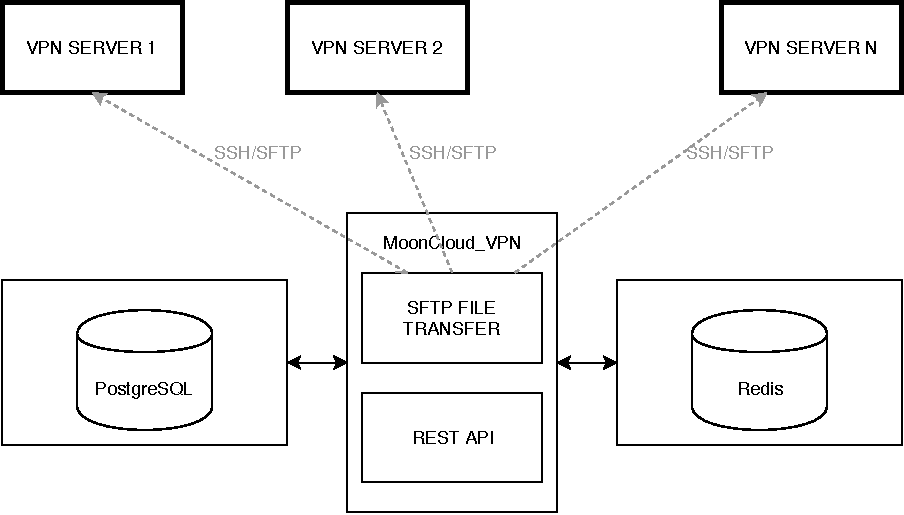
\includegraphics[scale=0.5]{img/microservice_deployment}
  \label{fig:microservice-deployment}
  \caption[Il deployment di \texttt{MoonCloud\_VPN}]{
    Il deployment di \texttt{MoonCloud\_VPN}. I rettangoli con linee in grassetto
    rappresentano le VM su cui vi sono i VPN server, mentre quelli con contorno
    normale rappresentano i tre container di cui il deployment si compone.
  }
\end{figure}


Il microservizio è composto da diversi moduli, ciascuno dei quali ben
specializzato per una certa funzionalità, ad esempio: creazione file di configurazione
server, creazione file per nftables, trasferimento file, ecc\ldots
Il modulo \texttt{controllers.py}  definisce
una serie di funzioni che, tramite \texttt{views.py} risponde direttamente alle
chiamate alle API del servizio. Si cura di chiamare i metodi delle classi di tutti
gli altri moduli.
% La figura \ref{fi}
% La figura \ref{fig:microservice-archi} mostra in maniera grafica i diversi moduli di cui
% si compone il microservizio, i quali sono descritti in maggior dettaglio di seguito.

\begin{description}
  \item[\texttt{client}]Questo modulo si occupa delle configurazioni relative ai
  client VPN. In particolare, contiene classi responsabili di creare il file
  di configurazione principale per un VPN client, creare i file client-specific
  da trasferire sul server, creare il file di script per nftables dato il mapping
  da usare per quel client.
  \item[\texttt{dnmcp}]Si occupa in maniera specifica di creare il mapping date
  le reti originali. Una volta che è stato definito, è responsabile di salvarlo
  nel database.
  \item[\texttt{dns}]Un modulo specifico dedicato alla risoluzione dei nomi
  DNS relative al blacklisting. Oltre a risolvere nuovi nomi ricevuti in input,
  è anche responsabile di aggiornare tutti quelli presenti nel database.
  La risoluzione viene fatta in maniera asincrona, ovvero si fanno tutte le query
  necessarie, una dopo l'altra senza aspettare risposta, e solo quando l'ultima
  è stata completata si aspettano i risultati complessivi. Questo consente
  di aumentare le performance mediante I/O non bloccante.
  \item[\texttt{openssl}]Una classe preposta alla creazione, revoca ed aggiornamento
  dei certificati di client e server, e gestione della CRL. Utilizza una
  libreria Python che a sua volta utilizza OpenSSL come backend.
  \item[\texttt{server}]L'unico compito dell'unica classe di questo modulo è quello
  di creare il file di configurazione principale per un VPN server, dati una serie
  di parametri in input.
  \item[\texttt{trans}]Il nome del modulo è l'abbreviazione di ``transfer''. Si
  compone di una serie di classi responsabili di trasferire file sui server mediante
  \texttt{sftp} (trasferimento file su un canale sicuro SSH) e di creare
  la struttura di directory così come assunta nel file di configurazione di OpenVPN
  (esempio: creare le cartelle \texttt{/etc/openvpn/\ldots/ccd/} e \texttt{/etc/openvpn/\ldots/certs}).
  \item[\texttt{workers}]Contiene la classe \texttt{SSHBackgroundWorker} la quale, mediante
  due thread separati, si occupa del trasferimento mediante il modulo \texttt{trans}.
  Maggiori dettagli su questa funzionalità verranno fornite in seguito durante
  il capitolo.
\end{description}

Infine si descrivono i seguenti moduli:
\begin{description}
  \item[\texttt{controllers}]Organizzato in dversi file, questo modulo si occupa di
  \textit{unire} le funzionalità messe a disposizione da tutti gli altri moduli,
  oltre a creare le istanze dei dati da memorizzare nel database.
  \item[\texttt{models}]Contiene la definizione delle tabelle memorizzate nel DBMS, secondo
  i cosidetti ``\texttt{Model}'' nella terminologia
  Django\footnote{\url{https://docs.djangoproject.com/en/2.1/topics/db/models/}}.
  \item[\texttt{views}]Definisce le API a cui il microservizio risponde, deserializza e serializza
  gli input e gli output, fà le chiamate a \texttt{controllers}, ne intercetta eventuali errori.
\end{description}